%!TEX root = ../bachelors_thesis.tex

\section{Model Overview}
For the implementation of this algorithm there was only one model that truly stood out in the sense of object orientated programming. For all other functions it proved rather difficult to find a clear class where it belonged to and also making good use of responsibilities of those classes. As mentioned in chapter \ref{chap: Justification Logic} the main work was done using syntax trees and so it was the most obvious class to build. I decided to make a extra class for the \emph{Nodes} where all the small things like setting a child, and checking if it is a root and such would be handled. \emph{Tree} and \emph{Node} could have been merge to be one class only but I found it easier to work with the code if the more standard and trivial stuff of binary trees was separated from what was more specific for this algorithm. A lot of the \emph{atomize} part is handled by the \emph{Tree} class since it works within the formula and also changes the structure of it.

The most important class however is the \emph{ProofSearch} class. It acts as a sort of main class as the initialization of the formula and the cs-list takes place here. It is also here that the methods of the \emph{Tree} class are called from. Its responsibility is to handle all algorithmic task that can be done without using a syntax tree. So the major logic of the conquer step is implemented here.

Last there is the typical \emph{Helper} class. The methods here are usually rather short  and simple and serve the purpose of making the \emph{Tree} and \emph{ProofSearch} class appear cleaner. It may be argued that some of those methods present in \emph{Helper} should be better placed in \emph{ProofSearch} and vice a verse but then again the argument for a clean object orientated model design for an algorithm is questionable and very difficult to archive.

\begin{figure}[H]
	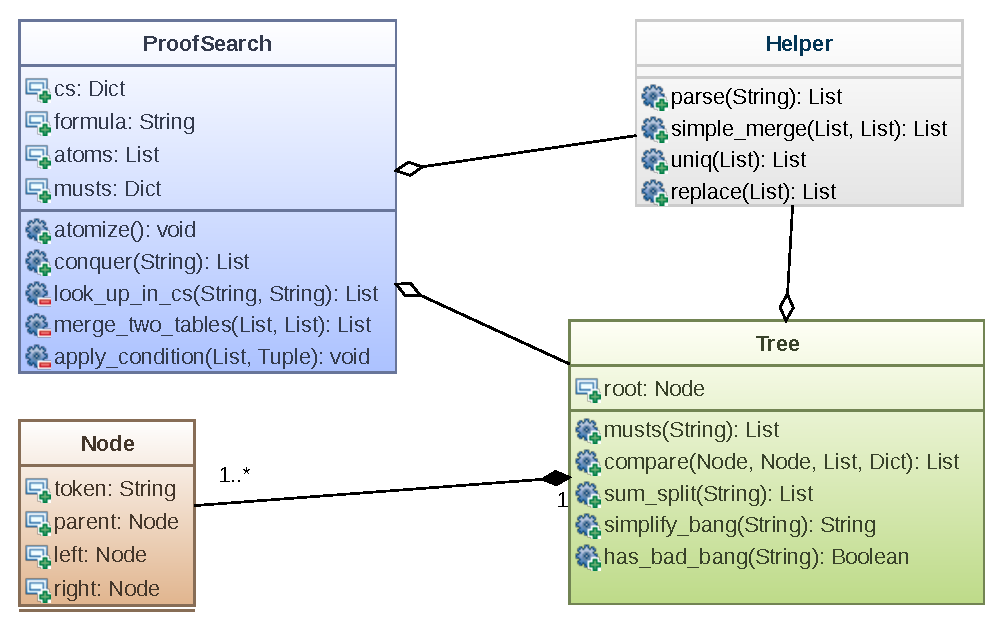
\includegraphics[width=0.9\textwidth]{/home/lyriael/BA/j-logic/thesis/Figures/uml_01.pdf}
	\caption{Simplified UML graphic of the classes used for implementing the algorithm. The list of methods and attributes is by no means complete and should simply give an idea of the construction.}
	\label{uml}
\end{figure}

\section{Operation Syntax Tree}
One of the earliest challenges was a useful representation of a formula with which I could work decently. Interestingly enough a binary tree came only later into my mind, after I tested various libraries from Python. There were libraries that seemed very useful at first as they were math-specific. Analyzing formulas that contained $*$ or $+$ were fairly easy but as $:$ and $!$ are not very common operations I could not customize the tested libraries enough to handle those as well.

So it happened while I was searching yet for another library that I tumbled over the possibility to use binary trees to represent the syntax of a mathematical formula. Remembering a lot of what I learned in the lecture about Datastructure and Algorithms I realized that this is the best choice for me. A binary tree gives me not only a way to represent a formula in a way that interprets the order of operations but with the knowledge about trees it became suddenly very easy to also manipulate such a formula for example by deleting or swapping subtrees and still keep a valid operation. 

I decided to implement my own tree for that purpose. It might be argued that a lot of work could be saved if I used available syntax trees but for one thing I relished the idea of implementing a tree structure that I would use myself and thus finally use what I have learned in lecture ages ago and second I would have to make custom changes to a finished solution anyway and those changes are probably more work than the implementation of a binary tree which is rather simple.

I tried to keep the tree as simple as possible, giving the nodes only a value and not a unique key. The greatest challenge given by implementing a syntax tree was to handle the unary operator $!$. As braces serve to determine the depth of a tree and a binary operation tells you when to start climbing up again, it required so extra case handling for the $!$ operator. From the point on when the tree was working, it was not only important to the algorithm, but could also be used to check if the input was written correctly. Therefore most of the tests that test the string handling of a tree are the result of formulas used somewhere else but which needed syntax spell checking. 


\section{Important Methods}
In this section I want to show and explain some of the more complicated methods that are important and make up the heart of the algorithm.

\subsection{musts}

The method \emph{musts} expects a given proof term to be already \emph{atomized} as it only distinguishes between $!$ and $*$ operations.
The algorithm takes the formula in form of a tree apart from top to bottom, generating new, smaller terms for every operation it takes apart until the remaining proof term is only a proof constant. Since the resolve of a $*$ operation needs a new \emph{X-wild} and the resolve of a $!$ operation replaces an existing \emph{x-wild} and therefore needs a new as well, the current $i$ for a new \emph{X-wild} $X_i$ is stored and increased in \texttt{v\_count}.

\begin{figure}[H]
    \vspace{-10pt}
	\lstinputlisting[firstline=2, lastline=22]{/home/lyriael/BA/j-logic/thesis/code_tree.py}
	\vspace{-10pt}
	\caption{Excerpt from $Tree.musts$}
	\vspace{-10pt}
\end{figure}

If for example the current justification term would be $((a*(!b)):F)$, it would be taken apart to the two subformulas $(a:(X_i\rightarrow F))$ and $((!b):(X_i))$. Because of the \emph{atomization} in the steps before it is guaranteed that every $!$ is a (right) child of a  $*$ and since every $*$ creates a new $X_i$, a term here that starts with a $*$ is always on a $X_i$. Since from $!b:X_i$ follows $\exists X_j \quad s.t. \quad !b:(b:X_j)$, all $X_i$ that occurred up to now must be replaced by $(b:X_j)$. In the end we will have only proof constants remaining.

\subsection{unify}
I spend probably most of my implementing time on this method, or rather on its predecessor. It used to be a lot longer and more complicated because it differentiated various cases if a formula would contain one or another kind of variable.
With this new and (hopefully) last implementation there is no different handling for \emph{X-wild} or \emph{Y-wild} variables on that level. Only much later when all results are put together will those variables be handled different accordingly.

The method is actually quiet forward: It takes two formulas\footnote{It is expected that the only occurring operations are $\rightarrow$ and $:$. It should be rather easy to extend the code at this point to accept also other operations but from what I can expect as input this is not necessary here.} and compares them on the basis of their tree structure. While the structure remains the same thus operations and constants match for both formulas the methods pushes the subtrees of both on the stack until either one of the subtrees consists only of a node containing a variable or a mismatch is found. In the later case \texttt{None} will be return the method is stopped. In the case that we find a node with a variable for one tree it will be formed into a \emph{condition} for that variable, where the variable is the key and whatever we find in the other tree at this place is the value.

\begin{figure}[H]
	\vspace{-10pt}
	\lstinputlisting[firstline=1, lastline=25]{/home/lyriael/BA/j-logic/thesis/code_formula_tools.py}
	\vspace{-10pt}
	\caption{Excerpt $unify$ from $FormulaTools$.}
	\vspace{-10pt}
\end{figure}

All those conditions are stored as tuples in a list and are returned in form of a dictionary, where all conditions for one variable can be accessed by the variable itself as key. At the current state conditions that apply to a variable may be contradictory, but it the responsibility of this method is only to collect those and not to valuate them. This is done by the method \texttt{simplify} and in a further extension also in the method \texttt{resolve\_conditions}.


\subsection{simplify}
This methods is used to get a result once all conditions are obtained by \texttt{unify}. The method is implemented in a way that it does only \emph{simplify} the conditions for \emph{one} Variable. To \emph{simplify} a whole set of variables with their conditions a very simple method called \texttt{resolve\_conditions} in \texttt{FormuaTools} is used. 

The aim of this method is that after it run there is only one condition term left for this variable and the variable itself does not occur anywhere else except as key to its condition. The reason behind this it that eventually we will have for every variable only one condition left. We would know for each variable what its value would be. As it is so often this idea proved harder to realize than first anticipated.

Where as I usually present here an excerpt from the original source code in the case of this method I rather present the idea in a more pseudo code manner since the source code contains a lot of indexing and parsing of data types that make it cumbersome to read and understand.

$X$ shall be our variable, and $F_1, F_2, ... F_n$ are all conditions that are mapped for this variable.

\begin{itemize}
	\item Preprocess all $F_i$: If any $F_i$ contains $X$ as part of its term we have a contradiction and the method will return \texttt{None} to indicate the contradiction. An exception is however if $F_i == X$ since this is not a very useful but a valid statement.
	\item For each pair $F_i$, $F_j$ we will use \texttt{unify} to check if those conditions are compatible. As we have seen above we will get a set of conditions again from \texttt{unify}. From the preprocess we are guarantied, that all those new conditions do not contain the variable $X$. If there is one pair of conditions that is not compatible the method will return \texttt{None} again to indicate the found contradiction.
	\item Choose one $F_k$ to be the only of the $F_n$ conditions to be put back in the set of original conditions. Since $F_k$ was matched with every other $F_i$ in the preceding step this one condition on $X$ together with the newly found conditions ensure that we don't loose any information and at the same time have only one condition on $X$ left.
	\item Replace all occurrences of $X$ in conditions of other variables with the single condition set to $X$ by the step above.
\end{itemize}

The steps above are those originally intended, while implementing it I found that there's a catch. The algorithm work fine the way it is described above for one variable but when iterating through all variables there was a problem because the conditions gained by \emph{unifying} the conditions of one variable might lead to new variable which where not present before because they only appear as part of a condition but not by themselves. The simplest solution seamed to be so initialize all variable and just leave the conditions empty, but because the order in which the variable are \emph{simplified} is not reliable it would be possible that a variable with no conditions is \emph{simplified} and only afterwards new conditions would be added. So the return value of this method is a list of the newly found variables. The condition set doesn't have to be returned since the changes are made in place.


So instead I worked recursively\footnote{To be precise I work with a stack and push any new variable on top so that it is next to be \emph{simplified}.} so that those new variables would be \emph{simplified} and thus replaced everywhere except a variable key and with one condition before the algorithm would randomly take the next variable to \emph{simplify}.


\subsection{conquer}
\todoWriteMore{Write about resolve conditions}


\section{Tests}
The tests I have written for this algorithm have been most important to the success of it. They served me in two ways: To check if my code would behave and actually do what I expected it to do and the other use was when I suddenly stumbled across a example or a situation where I did not know what I would expect I could see what my implementation would do with it, thus helping me to understand it better.
Of course blessing of the tests is also a curse as it is because of the tests that I found so many mistakes that I've made and forcing me to do it again and again.

As can be seen when looking at the source code not all all methods are tested on a same quality level. Methods that I deemed simple usually have only one or two tests. An example for that is \texttt{nice} from \texttt{ProofSearch}, this methods simply rearranges the elements of a dictionary and returns a nice readable output that summarized the content of the original input. In contrast to this methods are methods like the \texttt{conquer} methods and the \texttt{divide} method from \texttt{ProofSearch} or the \texttt{to\_s} from \texttt{Tree} which basically tests if the parsing between String and Tree works correctly.

To name some numbers, there are currently\footnote{Even though the program is finished it is still possible that I add more tests to get rid of any doubts, so the numbers are not fix.} a total of 66 tests. Almost halve of which are found in \texttt{ProofSearch}. 

As for the technology I used a simple unittesting framework.
